\documentclass[aspectratio=169]{beamer}
\usepackage{ngerman}
\usepackage[utf8]{inputenc} 

\usepackage{listings}
\usepackage{color}

\usetheme{Warsaw}  %% Themenwahl


\usepackage{pgfpages}
%\setbeameroption{show notes}
%\setbeameroption{show notes on second screen=right}
 
\title{Java Class Loading im Detail}
\author{Felix Becker}
\date{\today}
\institute{Scala Usergroup Köln}



\definecolor{javared}{rgb}{0.6,0,0} % for strings
\definecolor{javagreen}{rgb}{0.25,0.5,0.35} % comments
\definecolor{javapurple}{rgb}{0.5,0,0.35} % keywords
\definecolor{javadocblue}{rgb}{0.25,0.35,0.75} % javadoc
 
 \lstset{language=Java,
 basicstyle=\tiny,
 keywordstyle=\color{javapurple}\bfseries,
 stringstyle=\color{javared},
 commentstyle=\color{javagreen},
 morecomment=[s][\color{javadocblue}]{/**}{*/},
 numbers=left,
 numberstyle=\tiny\color{black},
 stepnumber=1,
 numbersep=10pt,
 tabsize=2,
 xleftmargin=1cm,
 showspaces=false,
 showstringspaces=false}


 
\begin{document}
\maketitle


\begin{frame}
	\frametitle{Vortragsinhalte}
	\tableofcontents
\end{frame}

\begin{frame}
	\frametitle{Motivation}
	\begin{itemize}
		\item{Grundlage für Vortrag von Mathias Kub}
		\item{ClassLoader-Hölle bei vielen Entwicklern gefürchtet}
		\item{Verständnis vom class loading bei komplexen Fehlersituationen notwendig}
		\item{Vorbereitung für Folgetalks über Scala Bytecode / JVM Internals + Scala}
	\end{itemize}
\end{frame}

\section{Class Loading Grundlagen}

\begin{frame}
	\frametitle{Was tun ClassLoader eigentlich?}
	\begin{itemize}
		\item{Laden Klassen und Resourcen aus beliebigen Quellen}
		\item{Trennen die Datenquelle von der Applikation, Applikation muss nur den ClassLoader nutzen (Plattformunabhängigkeit!)}
		\item{Klassen werden im JVM-Bytecode-Format geladen}
		\item{Resourcen können beliebige Daten sein}
	\end{itemize}
\end{frame}

\subsection{Class startup life cycle}

\begin{frame}
	\frametitle{Startup life cycle einer Javaklasse (JVM Spec §12.1.2)}
	\begin{enumerate}
		\item{Loading §12.2.1}
			\begin{itemize}
				\item{Laden des Bytecodes in die JVM über den ClassLoader}
			\end{itemize}
		\item{Verify §12.3.1}
			\begin{itemize}
				\item{Validierung der Klassenstruktur / Daten (Opcodes gültig, branch instructions check, signature check, ...)}
			\end{itemize}
		\item{Prepare §12.3.2}
			\begin{itemize}
				\item{Storage Allocation, Initialisierung von static fields (default values, keine static Initializer)}
			\end{itemize}
		\item{(Resolve §12.3.3)}
			\begin{itemize}
				\item{Optionaler Schritt - Symbolic link resolution}
			\end{itemize}
		\item{Initialization §12.4.1}
			\begin{itemize}
				\item{Aufruf von Static-Initializern, Initialisierung von static fields}
			\end{itemize}
	\end{enumerate}
\end{frame}

\begin{frame}
	\frametitle{Initialization}
	Initialisierung der Klasse ist die erste ''aktive'' Codeausführung von Klassencode (falls static fields / initializers vorhanden). Initialisierung findet statt, wenn das erste Mal:
	\begin{itemize}
		\item{eine Instanz der Klasse erstellt wird}
		\item{eine static-Methode der Klasse aufgerufen wird}
		\item{auf static-Variablen der Klasse zugegriffen wird (Zuweisung, Lesen)}
	\end{itemize}

	Die Initialisierung einer Klasse erzwingt die Initialisierung aller Super-Classes (gilt nicht für Interfaces!)
	\pause
	\begin{block}{Initialisierungen sind Threadsafe - sichere Erzeugung von Singletons!}
		Die Initialisierung ist intern in der JVM über ein initialization lock abgesichert. Die JVM garantiert, dass die Initialisierung einer Klasse genau 1x stattfindet. 
	\end{block}
\end{frame}

\subsection{ClassLoader delegation model}

\begin{frame}
	\frametitle{Standard-ClassLoader JVM 8 (Oracle)}
	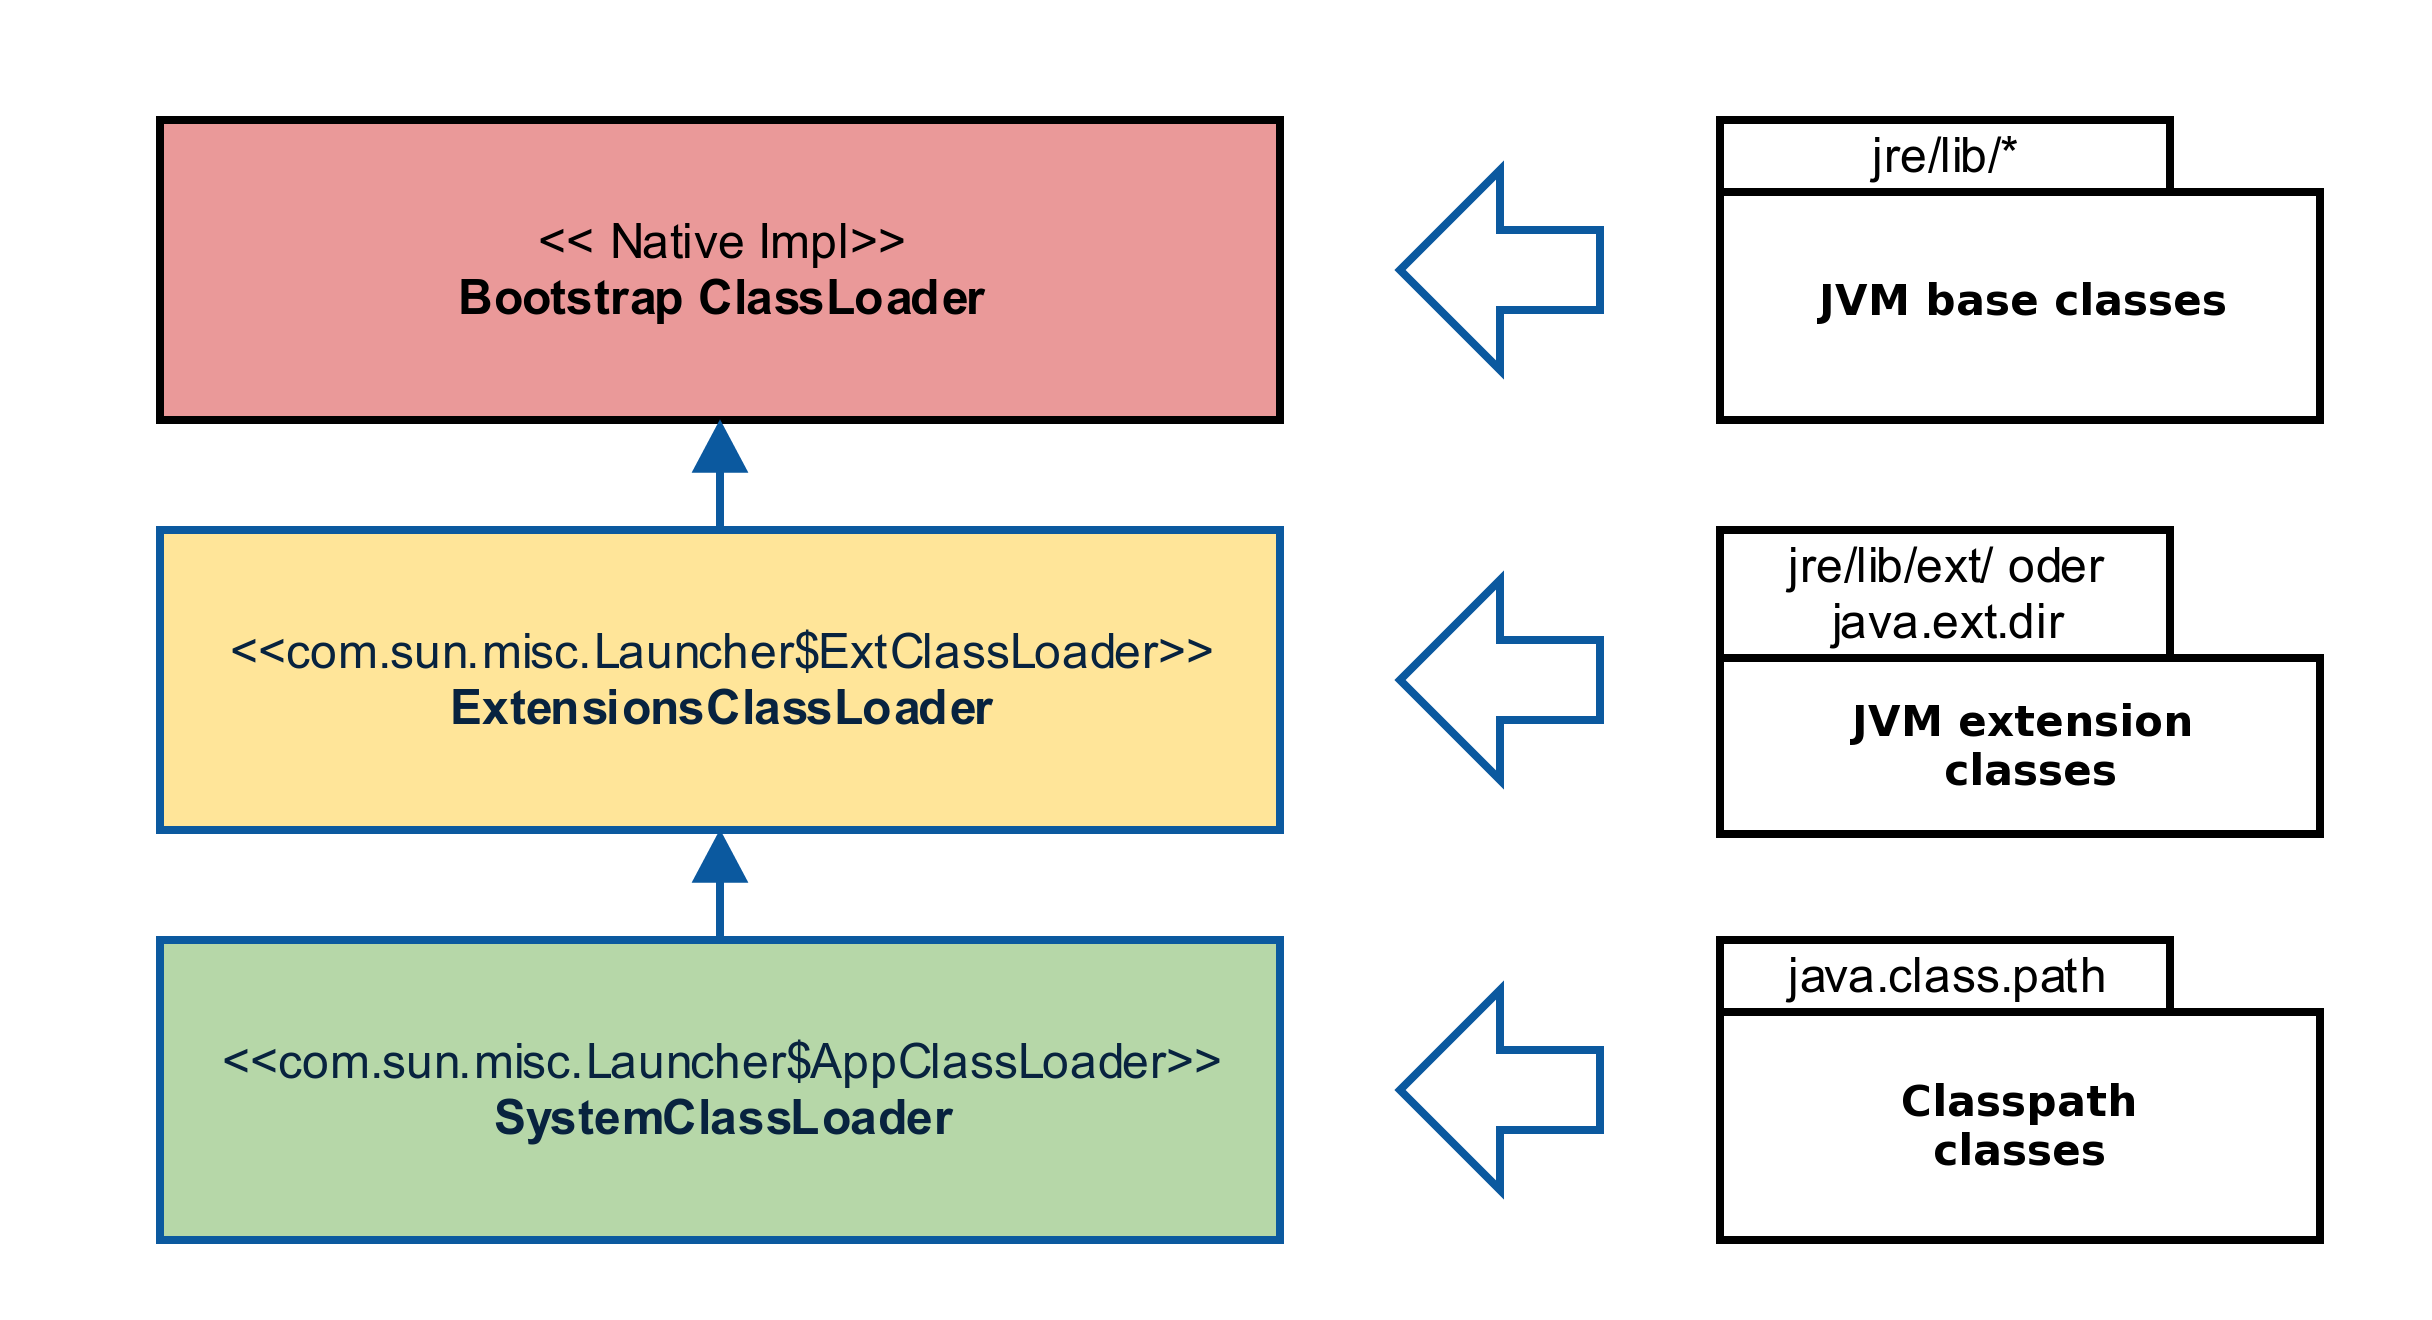
\includegraphics[scale=0.1]{assets/classloader-hierachie.png} 
\end{frame}

\begin{frame}
	\frametitle{Bootstrap-ClassLoader}
	\begin{columns}[T] 
	\begin{column}{.46\textwidth}
		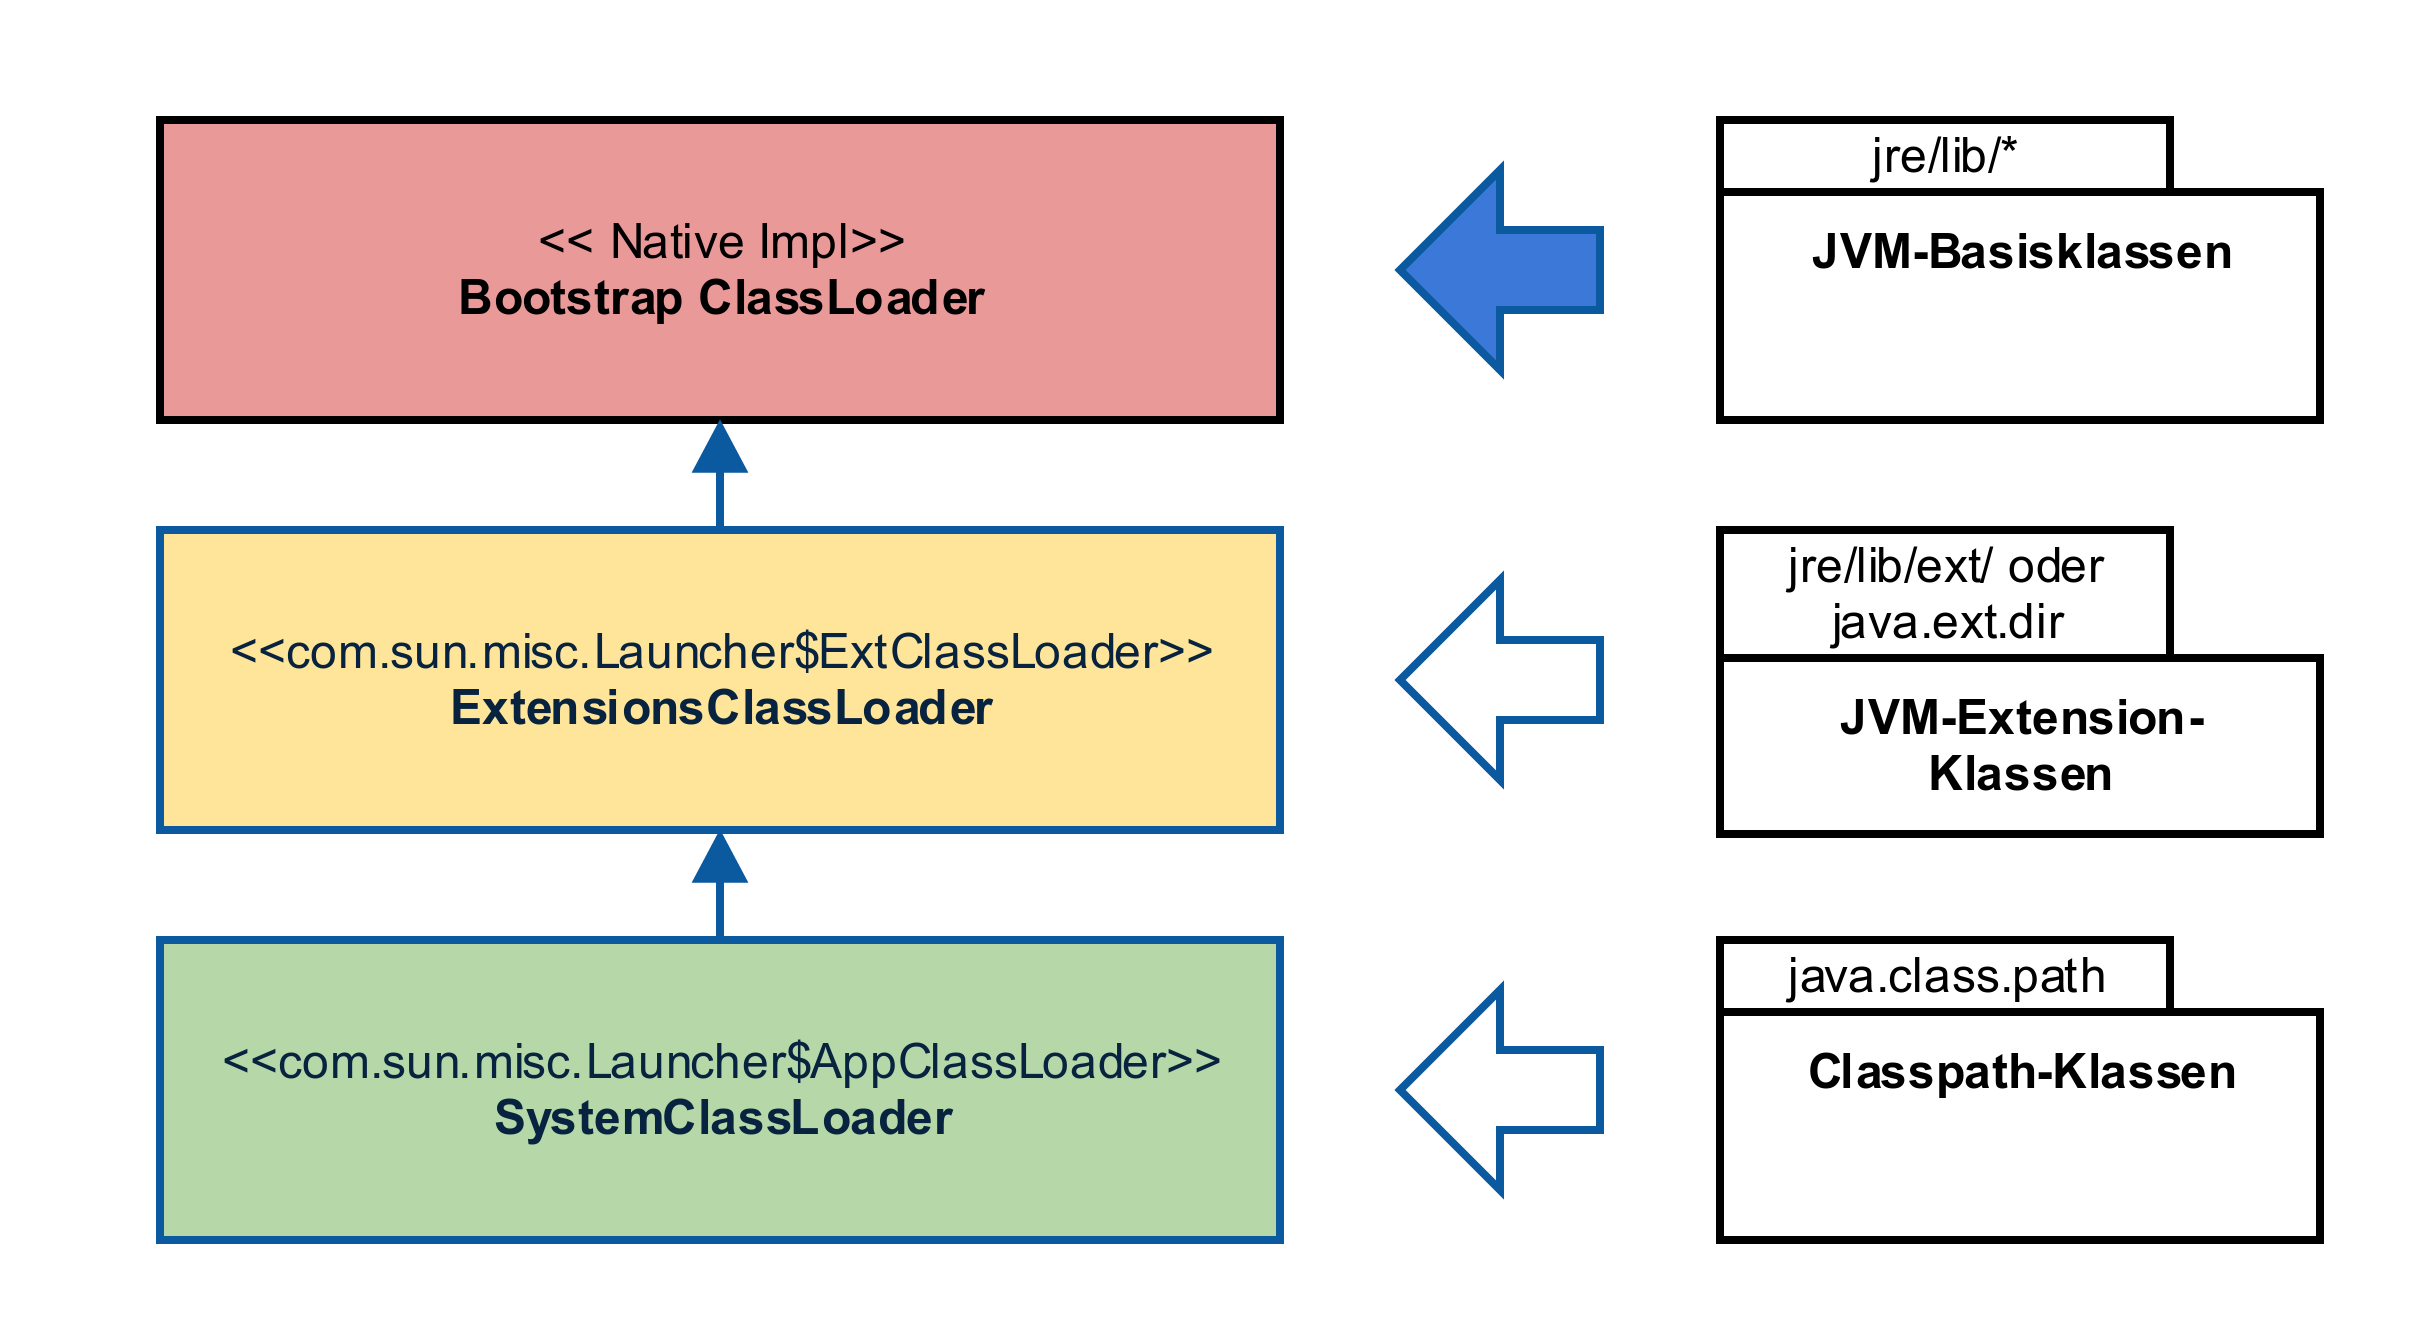
\includegraphics[scale=0.06]{assets/classloader-hierachie-bootstrap-active.png} 
	\end{column}
	\hfill
	\begin{column}{.56\textwidth}

	\begin{itemize}
		\item{Lädt Java-Basisklassen (z.B. java/lang/String)}
		\item{Nativ implementiert}
		\item{java.lang.ClassLoader: private nativ Class findBootstrapClass}
	\end{itemize}

	\end{column}
	\end{columns}
\end{frame}

\begin{frame}
	\frametitle{Extension-ClassLoader}
	\begin{columns}[T] 
	\begin{column}{.46\textwidth}
		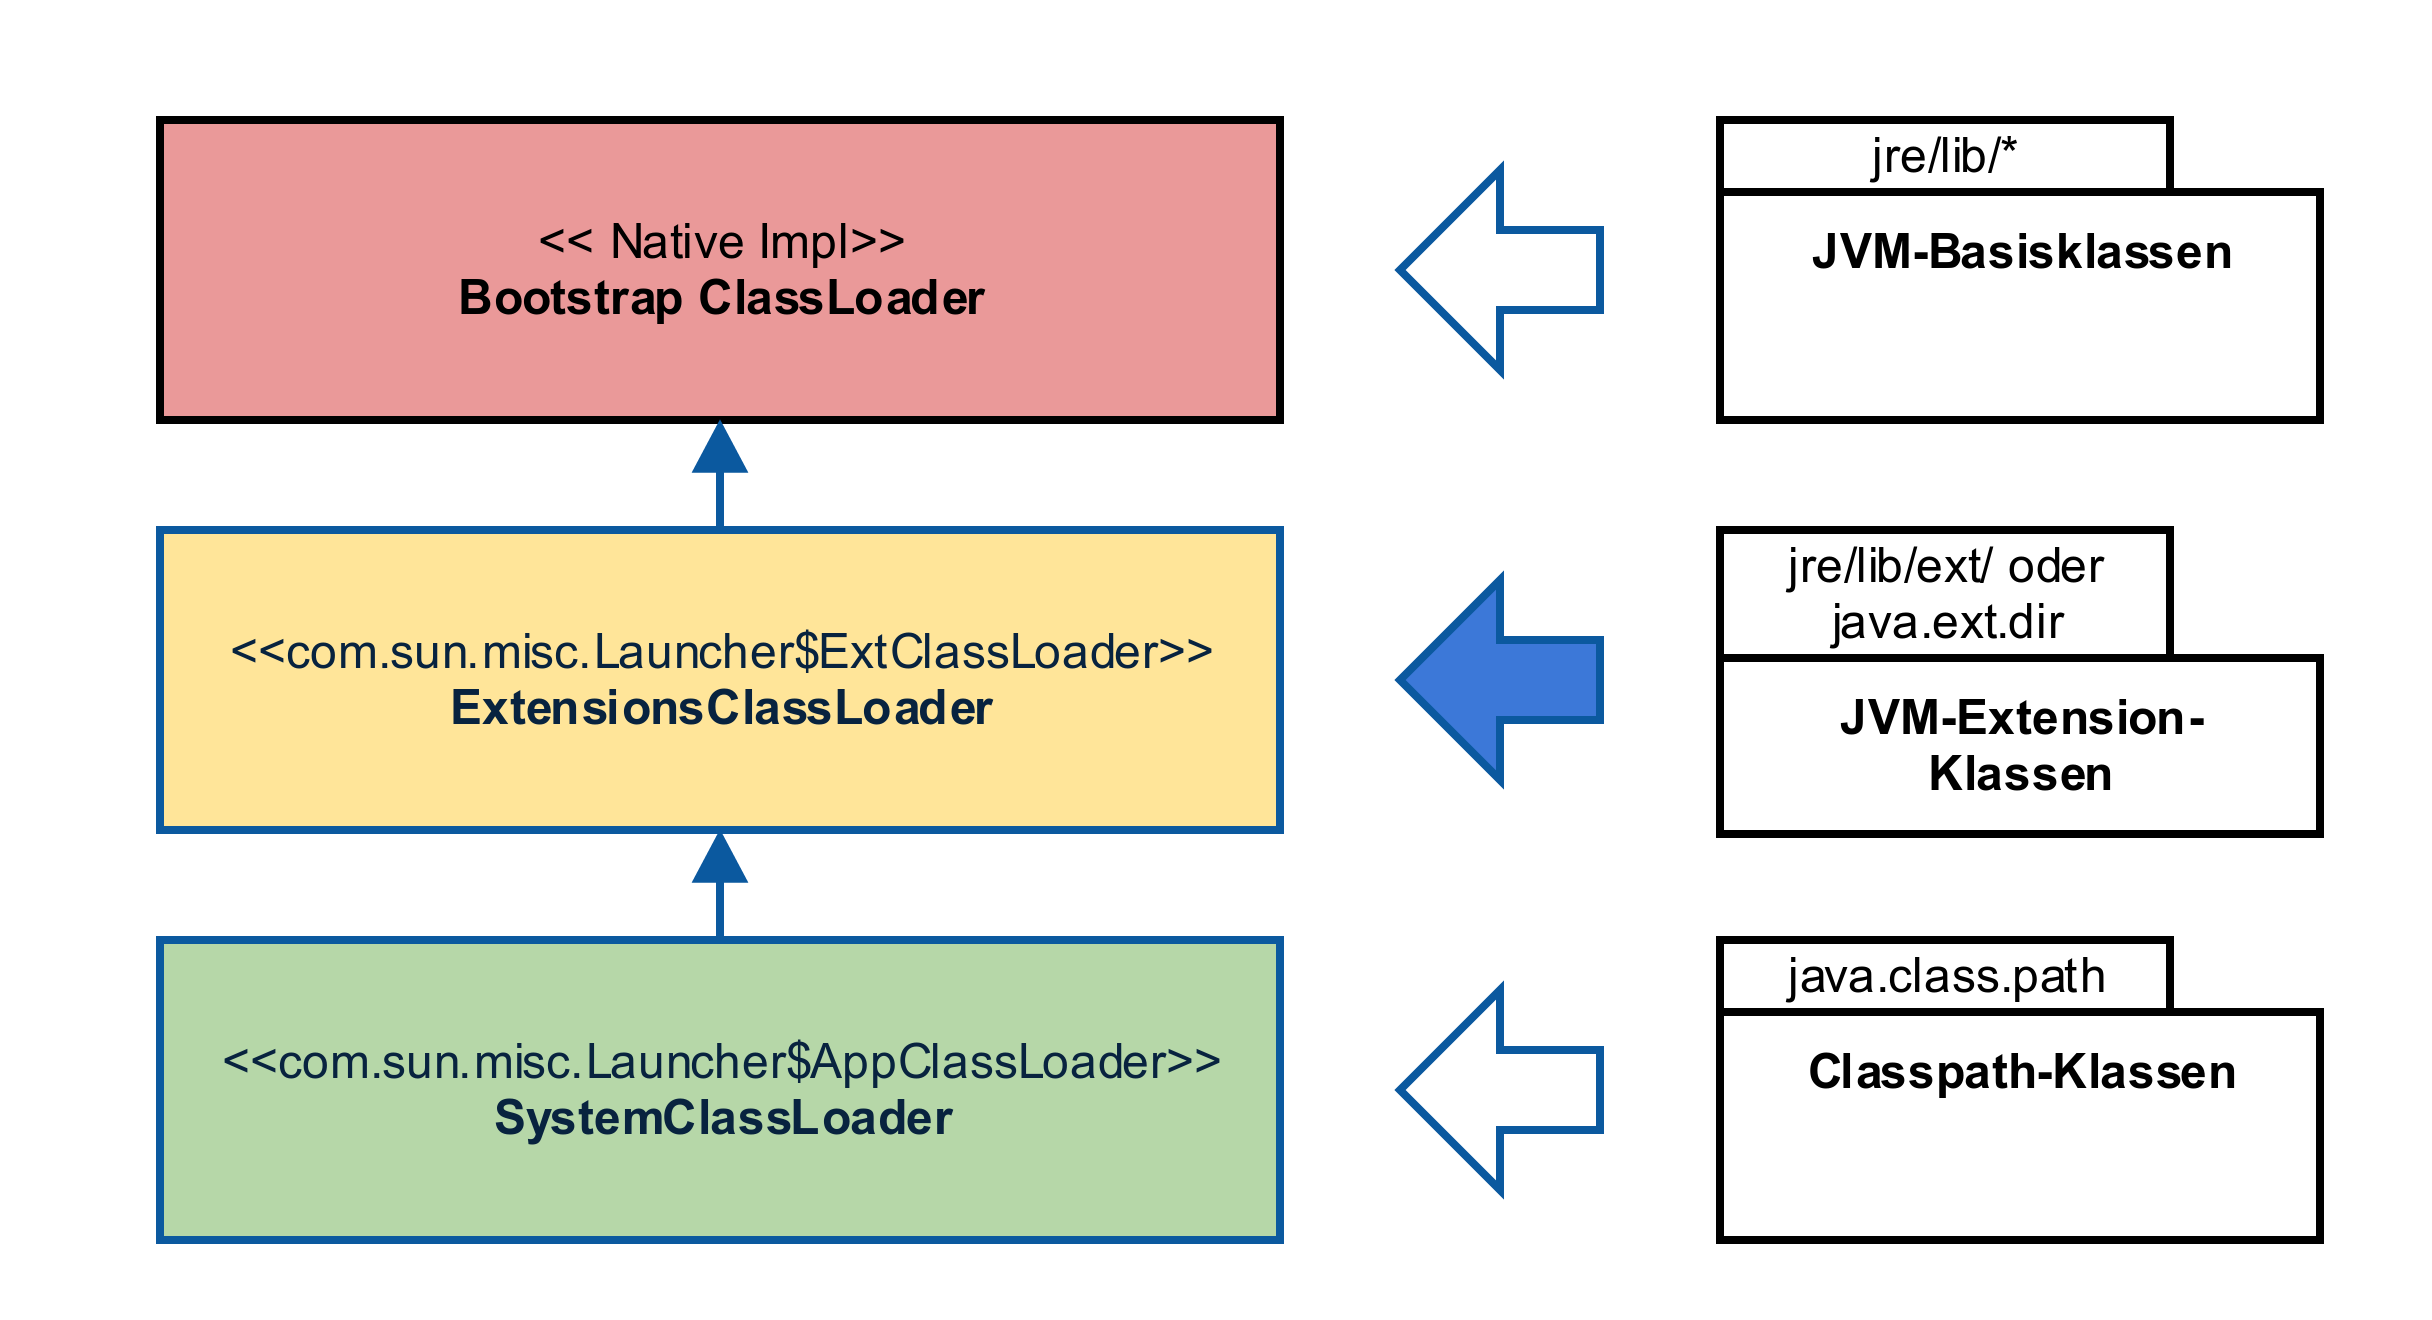
\includegraphics[scale=0.06]{assets/classloader-hierachie-extension-active.png} 
	\end{column}
	\hfill
	\begin{column}{.56\textwidth}

	\begin{itemize}
		\item{Lädt Extension-Klassen}
		\item{Beispiel: com/sun/nio/zipfs/ZipPath}
		\item{lädt Extension-Klassen aus jre/lib/ext/ bzw. java.ext.dirs}
		\item{com.sun.misc.Launcher\$ExtClassLoader}
	\end{itemize}
	\end{column}
	\end{columns}
\end{frame}

\begin{frame}
	\frametitle{System-ClassLoader}
	\begin{columns}[T] 
	\begin{column}{.46\textwidth}
		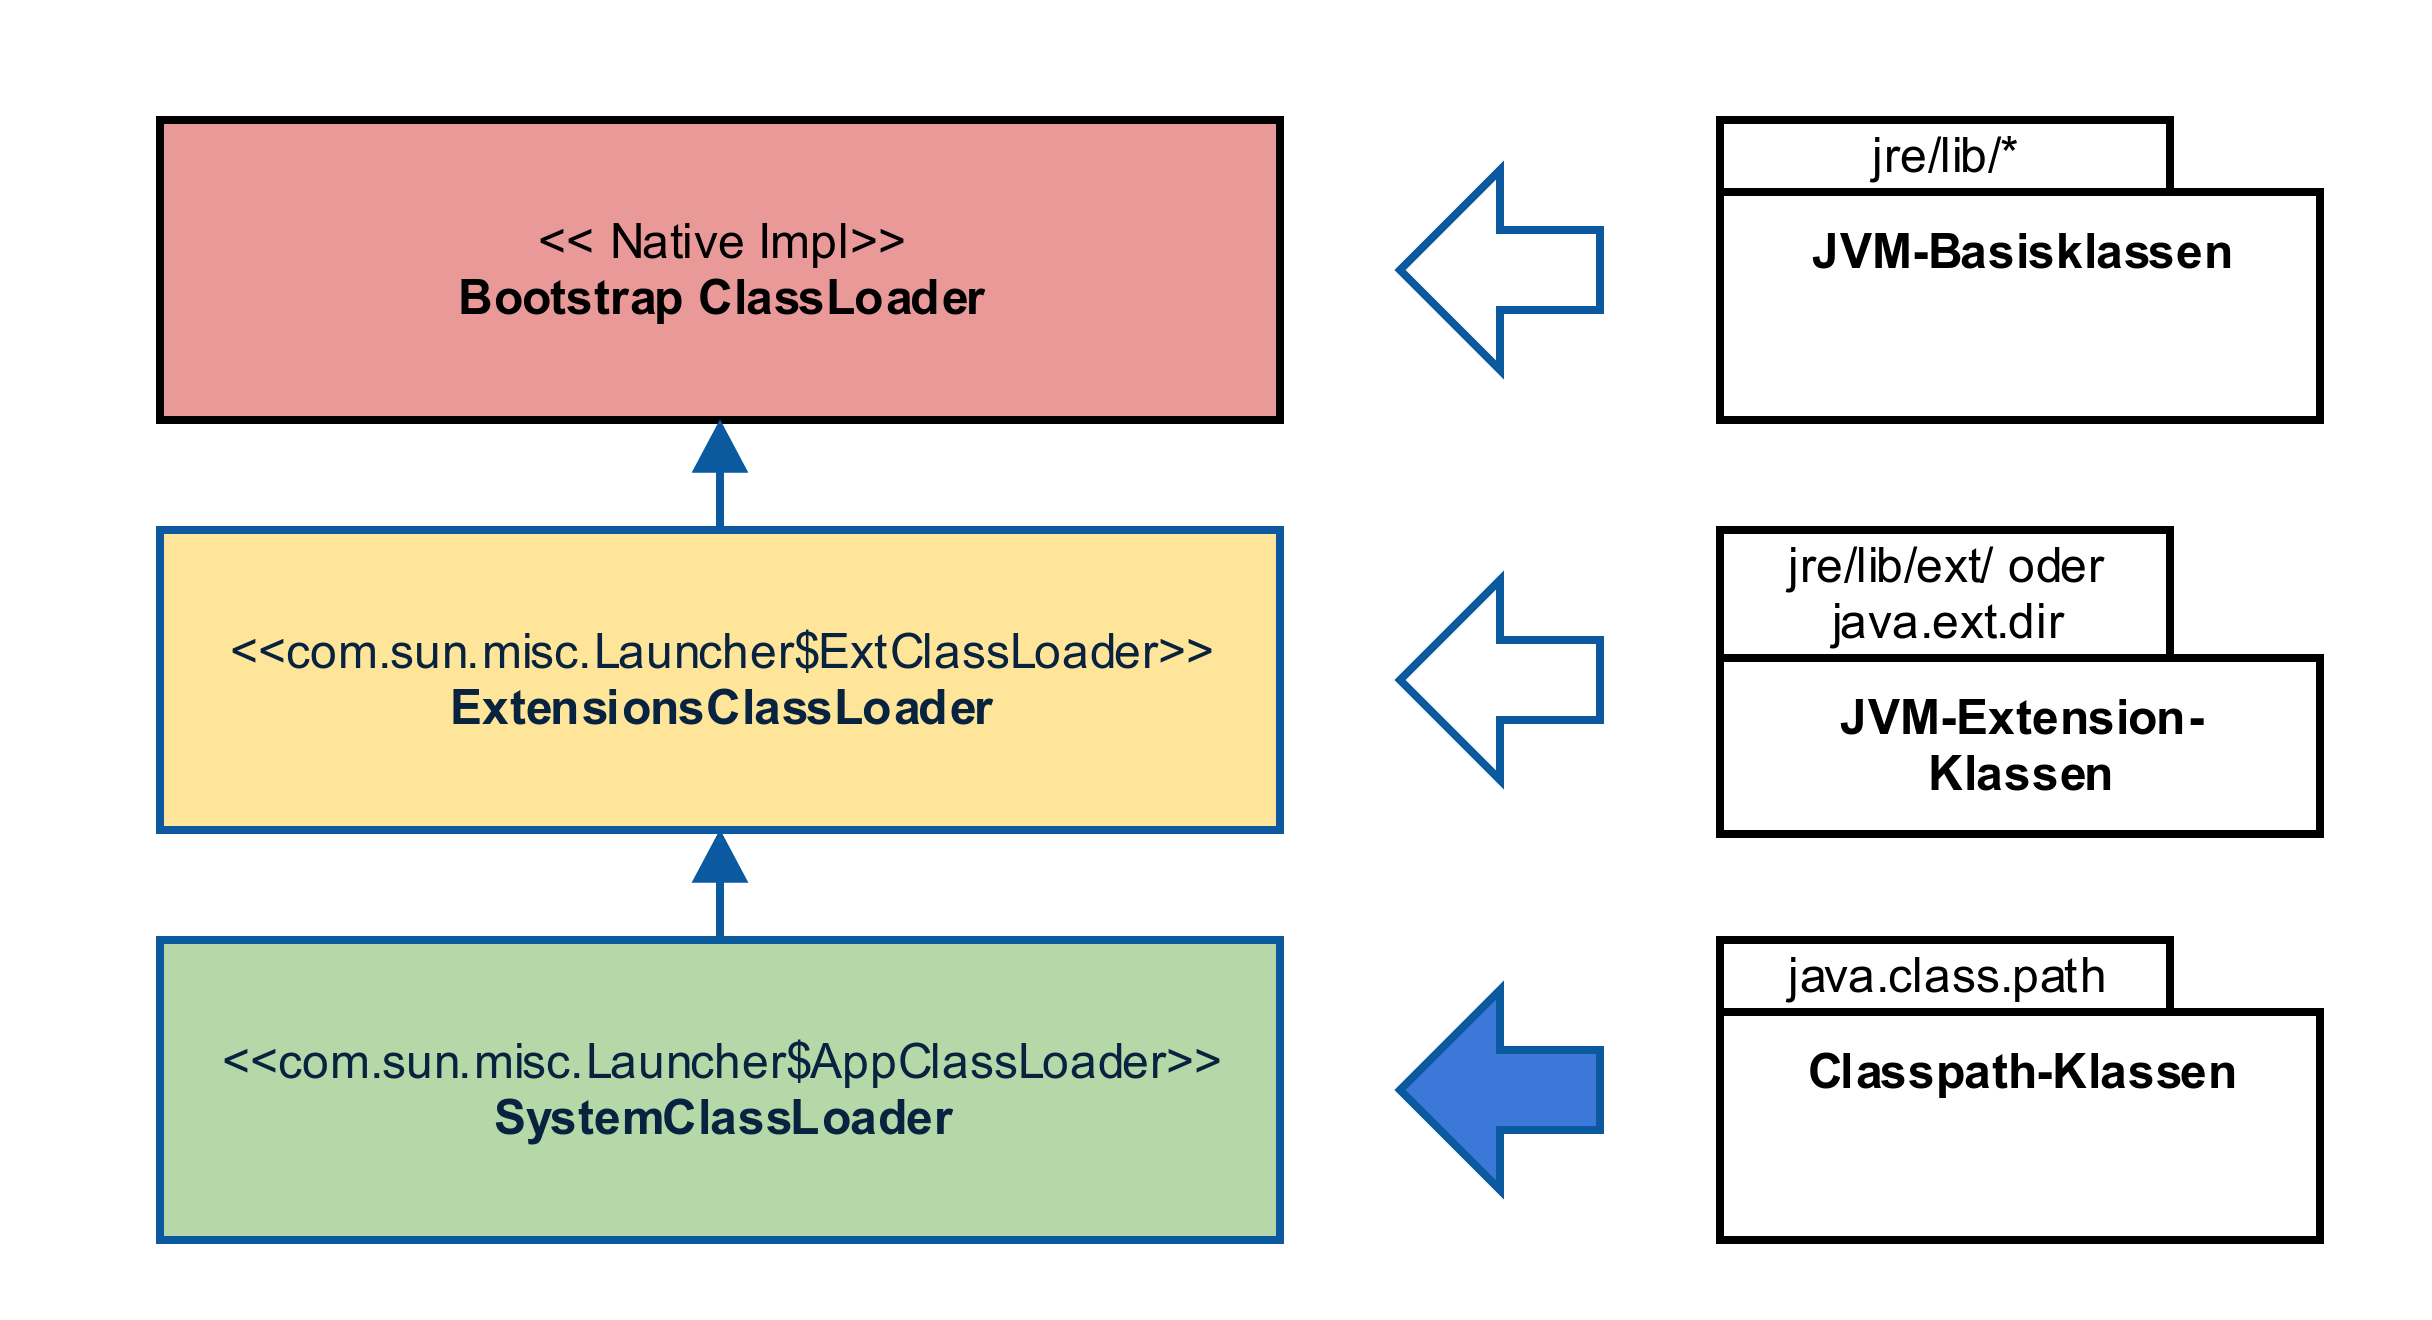
\includegraphics[scale=0.06]{assets/classloader-hierachie-system-active.png} 
	\end{column}
	\hfill
	\begin{column}{.56\textwidth}

	\begin{itemize}
		\item{Lädt alle Klassen aus dem java.class.path (java -cp ..)}
		\item{java.class.path (com.sun.misc.Launcher\$AppClassLoader)}
	\end{itemize}

	\end{column}
	\end{columns}
\end{frame}

\section{ClassLoader-Implementierungen}

\begin{frame}
	\frametitle{Relevante Funktionen}
	\begin{itemize}
		\item{Aus Applikationssicht:}
			\begin{itemize}
				\item{Class.forName(String)}
				\item{Class.getClassLoader()}
				\item{ClassLoader.loadClass(String)}
			\end{itemize}
		\item{Im ClassLoader:}
			\begin{itemize}
				\item{findLoadedClass(String)}
				\item{findBootstrapClassOrNull(String)}
				\item{resolveClass}
				\item{defineClass}
			\end{itemize}
	\end{itemize}
\end{frame}

\begin{frame}
	Live-Demo 1: First Steps
\end{frame}

\begin{frame}
	\frametitle{resolveClass Kuriositäten}
	'protected Class\textless?\textgreater loadClass( String name, boolean resolve ) Lädt die Klasse und bindet sie mit resolveClass() ein, wenn resolve gleich true ist.'
	WTF?
	\lstinputlisting{jvm-resolveclass.cpp}
\end{frame}

\begin{frame}
	\frametitle{ClassLoader.loadClass}
	\begin{columns}[T] 
		\begin{column}{.57\textwidth}
			\lstinputlisting{ClassLoaderLoadClass.java}
		\end{column}
		\hfill
		\begin{column}{.43\textwidth}
			\begin{itemize}
				\item{Class Loading ist synchronized}
				\item{Lookup-Schritte:}
				\begin{enumerate}
				\item{findLoadedClass (native)}
				\item{parent / bootstrap lookup}
				\item{findClass}
				\end{enumerate}
				\item{findClass wird von eigenen ClassLoader-Implementierungen überschrieben}
			\end{itemize}
		\end{column}
	\end{columns}
\end{frame}

\begin{frame}[fragile]
	\frametitle{ClassLoader.getResource}
	\begin{columns}[T] 
		\begin{column}{.50\textwidth}
			\lstinputlisting{ClassLoaderGetResource.java}
	\end{column}
	\hfill
	\begin{column}{.50\textwidth}
			\begin{itemize}
				\item{Zuerst wird beim Parent / Bootstrap-ClassLoader nach der Resource gesucht}
				\item{findResource wird aufgerufen, falls Parent / Bootstrap keine Resource gefunden haben}
				\item{findResource wird von eigenen ClassLoader-Implementierungen überschrieben}
			\end{itemize}
		\end{column}
	\end{columns}
\end{frame}

\begin{frame}
	\frametitle{URL-ClassLoader}
	\lstinputlisting{URLClassLoaderFindClass.java}
\end{frame}

\begin{frame}
	Live-Demo 2: URL-ClassLoader
\end{frame}
 
\section{Fortgeschrittene ClassLoader-Techniken}


	\subsection{Der ContextClassLoader \& die WebApps}
	\begin{frame}
		\frametitle{WebApp ClassLoader}
		\begin{center}
			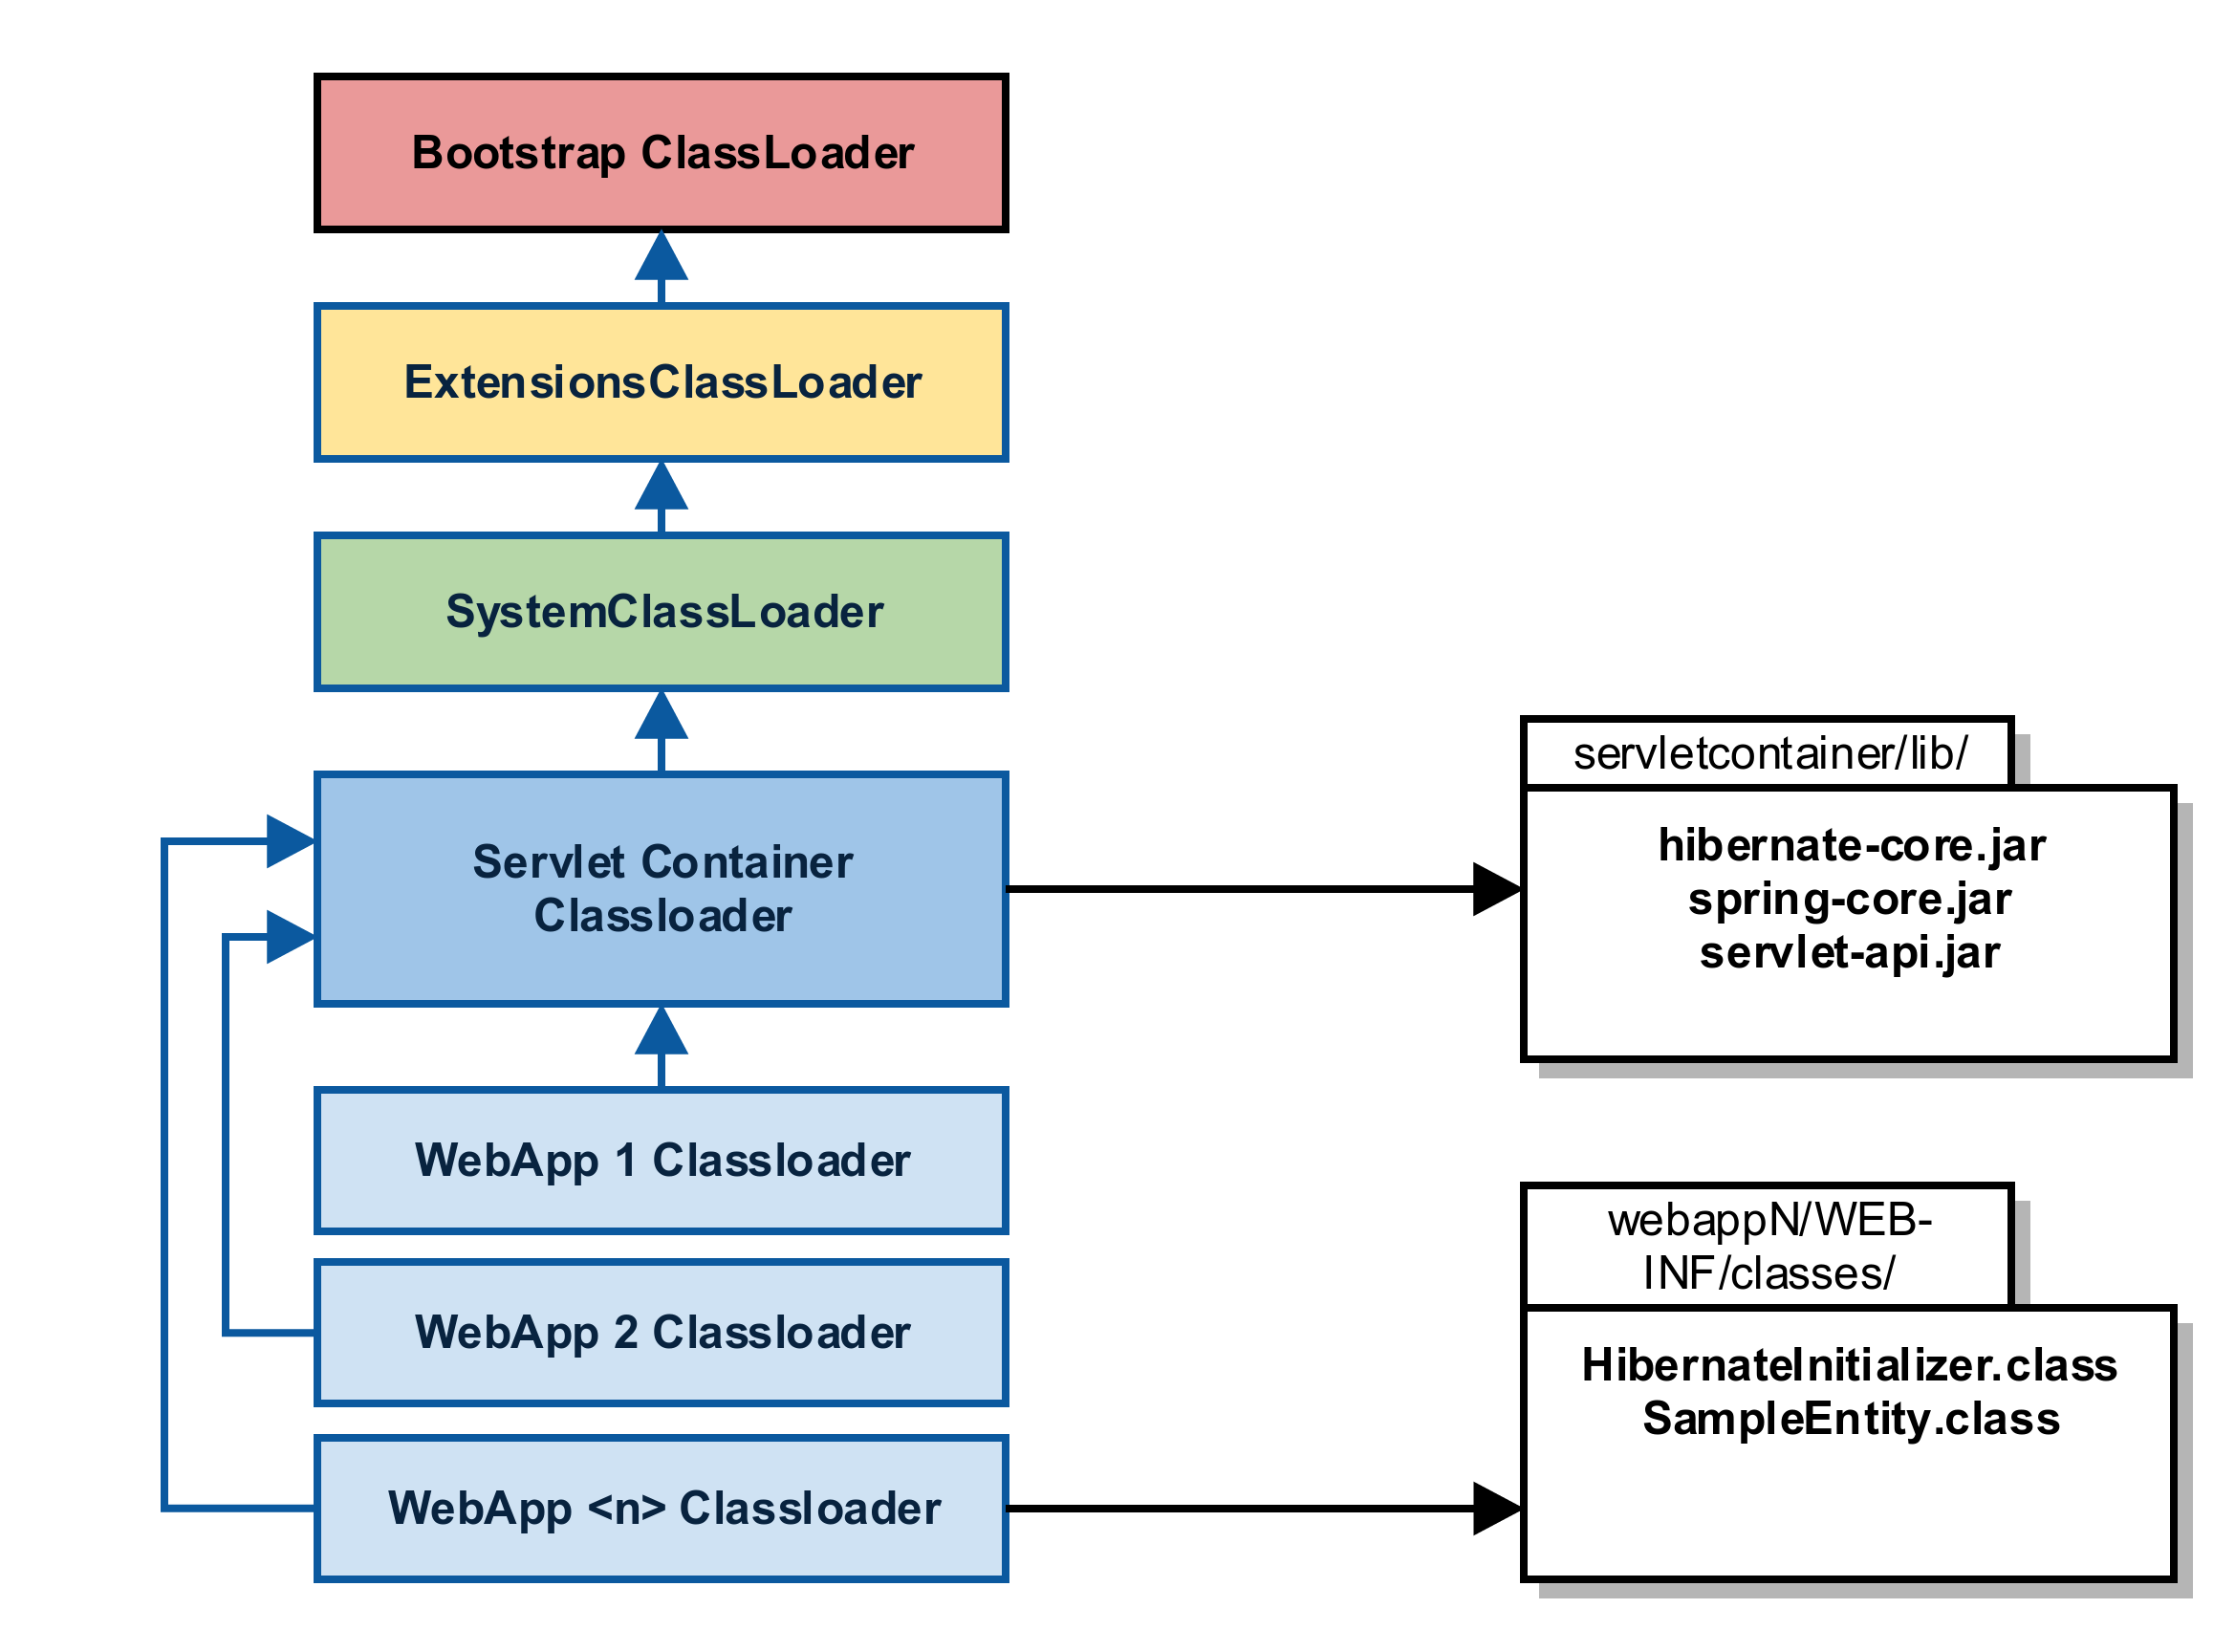
\includegraphics[scale=0.1]{assets/contextclassloader/webappclassloader-1.png} 
		\end{center}
	\end{frame}
	\begin{frame}
		\frametitle{WebApp ClassLoader - Context ClassLoader}
		\begin{center}
			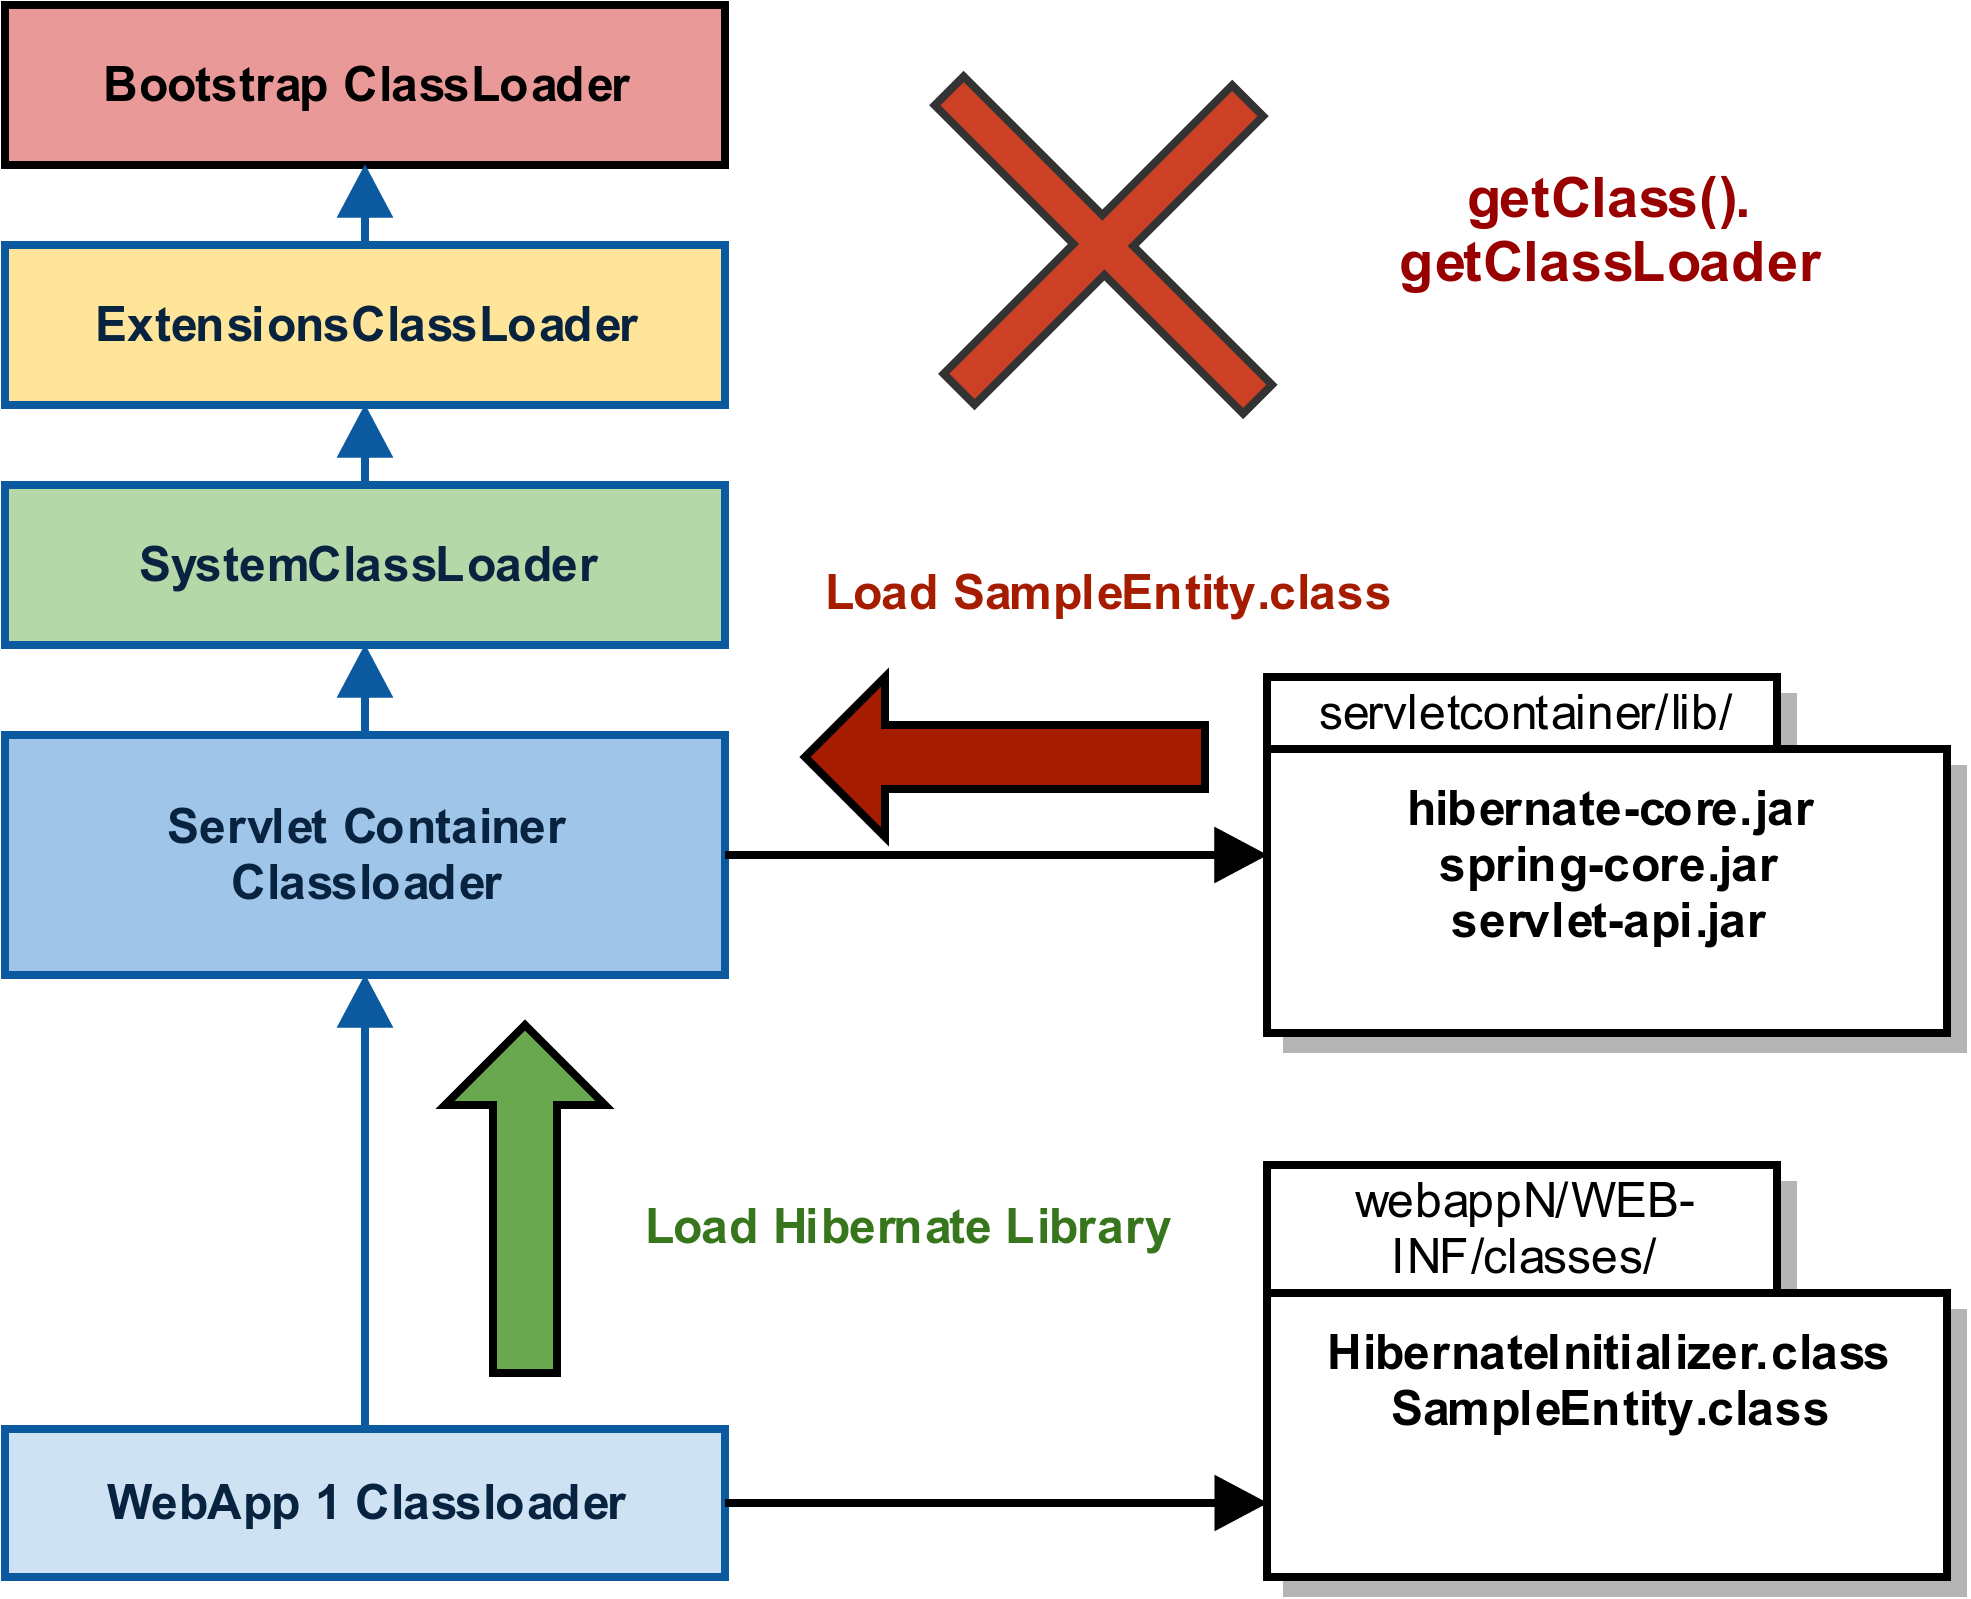
\includegraphics[scale=0.1]{assets/contextclassloader/webappclassloader-2.png} 
		\end{center}
	\end{frame}
	\begin{frame}
		\frametitle{WebApp ClassLoader - Context ClassLoader}
		\begin{center}
			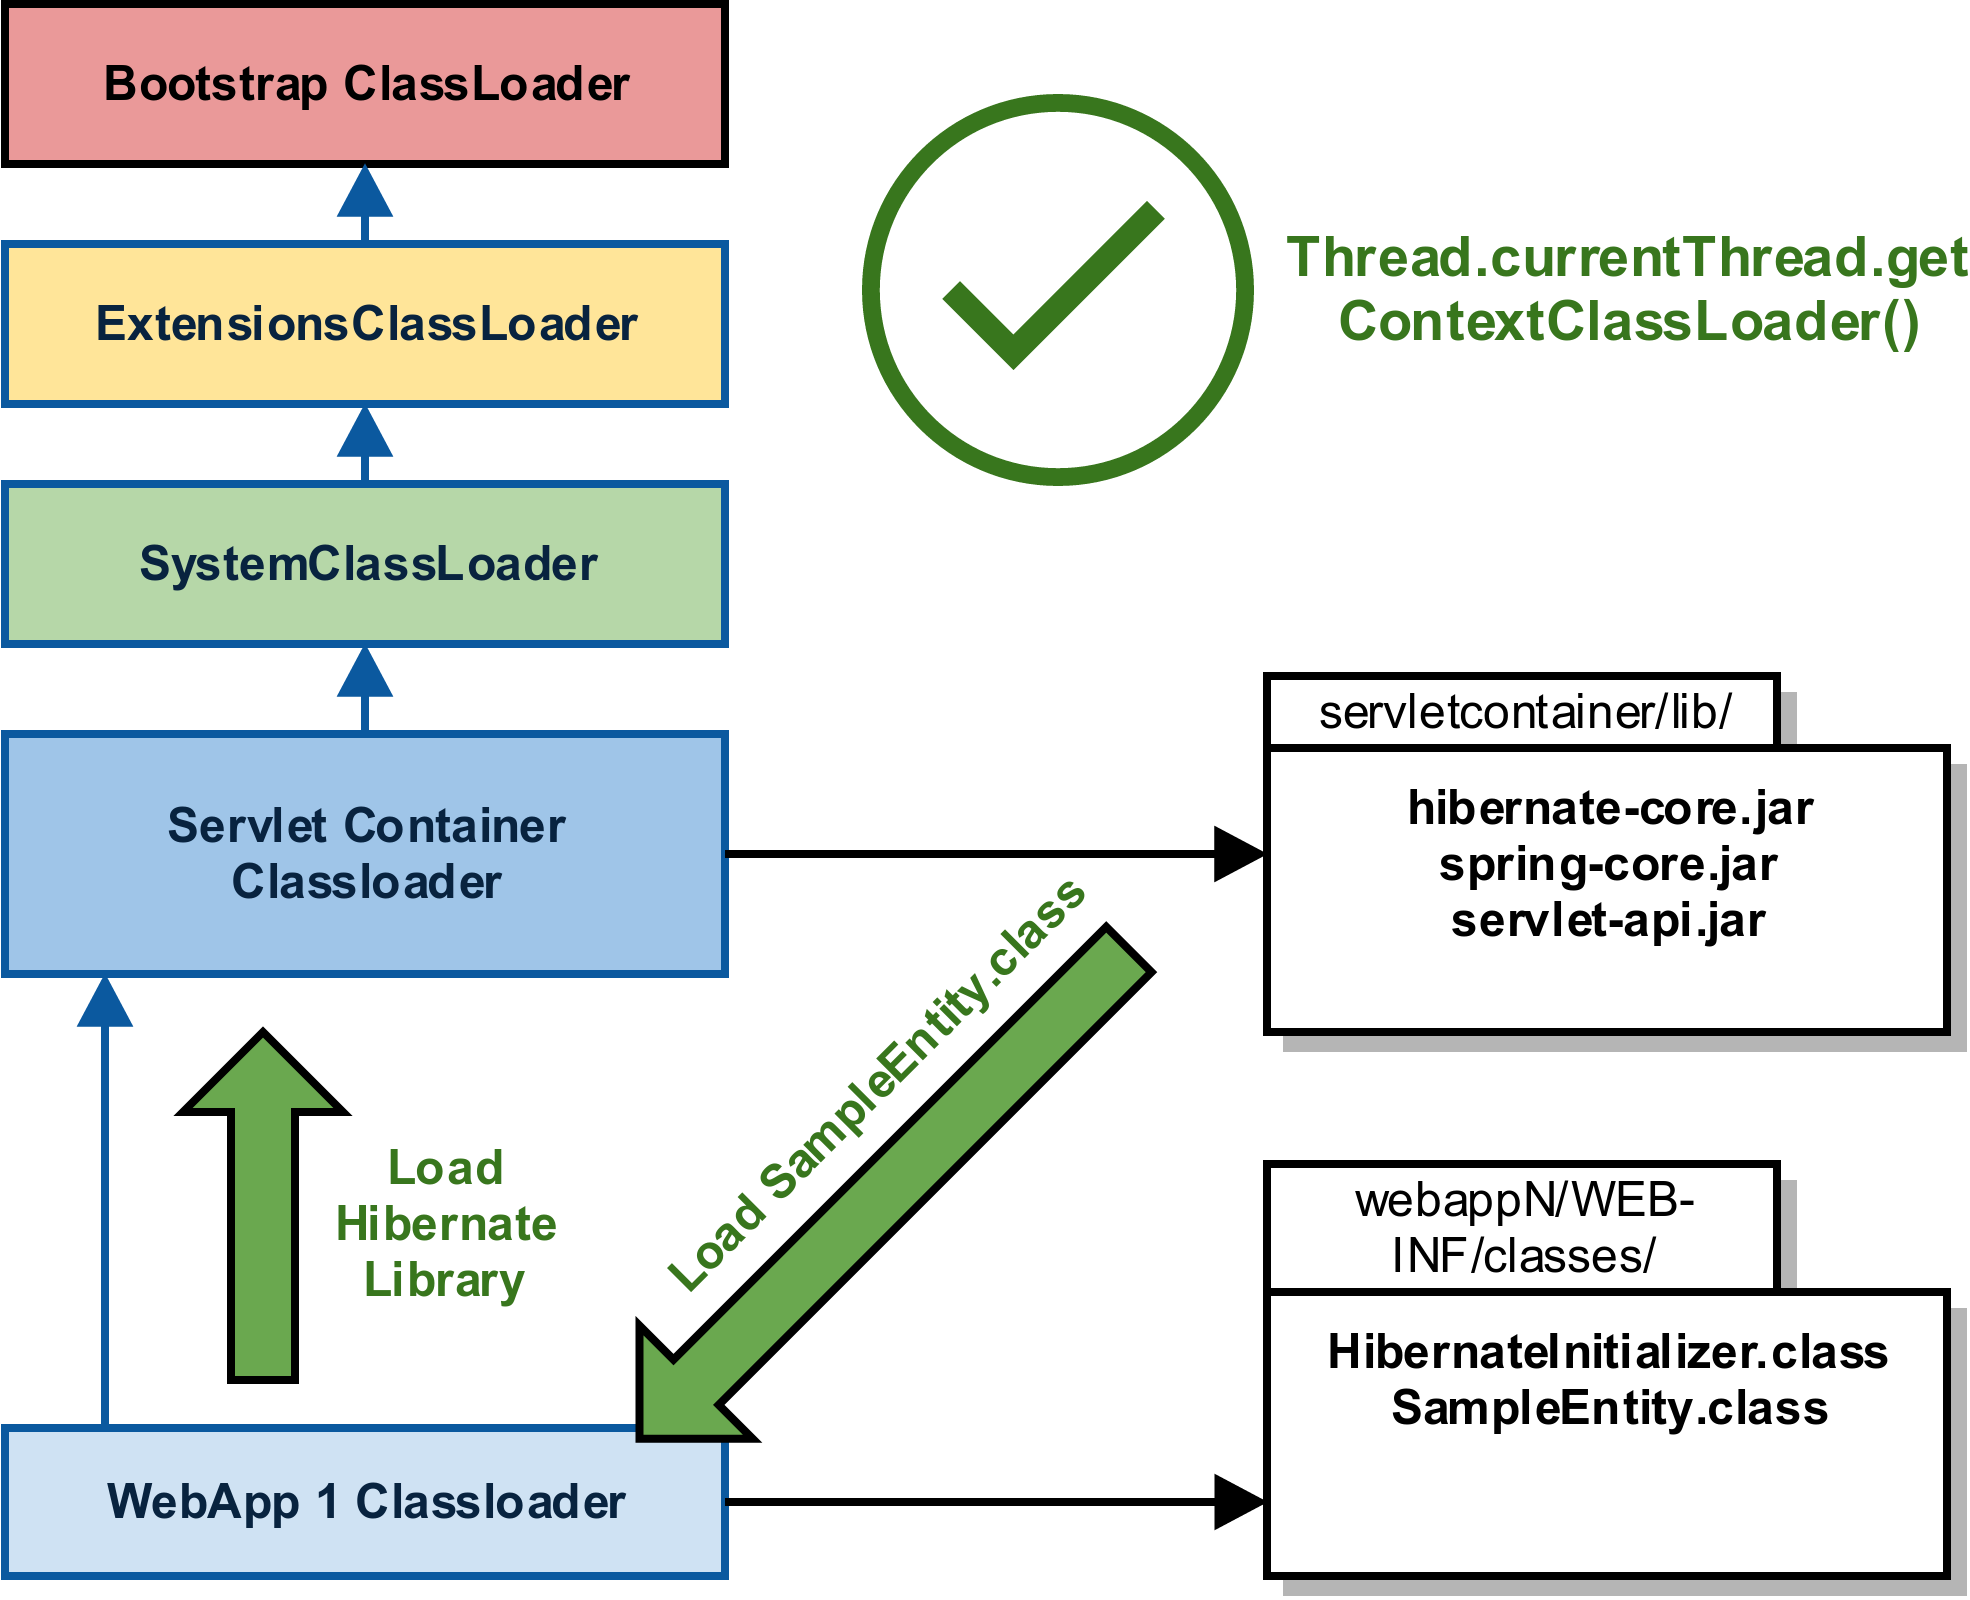
\includegraphics[scale=0.1]{assets/contextclassloader/webappclassloader-3.png} 
		\end{center}
	\end{frame}

	\begin{frame}
		Live-Demo 3: Doppeltes Laden von Klassen über getrennte ClassLoader
	\end{frame}

	\subsection{Loading Synthetic Classes}

	\begin{frame}
		\frametitle{Synthetic Classes}
		\begin{itemize}
			\item{Synthetische Klassen sind ''künstliche'' Klassen, die nicht im source code abgebildet werden}
			\item{Werden vom Compiler oder zur Runtime erzeugt}
			\item{Stark eingesetzt im AOP-Umfeld - z.B Transaktions-Proxy-Klassen}
			\item{Nutzung in Testframeworks wie PowerMock}
			\item{Können neben dem Proxy-API von Java auch aus Bytes direkt im ClassLoader erzeugt werden}
		\end{itemize}
	\end{frame}

	\begin{frame}
		Live-Demo 4: Erzeugung synthetischer Klassen
	\end{frame}

	
	\begin{frame}
		\frametitle{Ende}
		
		\begin{center}
			Vielen Dank für eure Aufmerksamkeit!
			\par
			Vortrag und Sourcen auf \href{https://github.com/fbe/classloader-vortrag}{github.com/fbe/classloader-vortrag}
		\end{center}

	\end{frame}

\end{document}

